\documentclass{article}
\usepackage[utf8]{inputenc}
\usepackage{graphicx}
\usepackage{xcolor}
\definecolor{mydarkgray}{RGB}{55, 55, 55}
\definecolor{mydarkviolet}{RGB}{102, 0, 153}
\usepackage[hidelinks, colorlinks=true, linkcolor=mydarkviolet, urlcolor=mydarkviolet, citecolor=cyan]{hyperref}
\usepackage{listings}
\usepackage{ragged2e}  
\usepackage{float}
\usepackage{url} 
\usepackage{animate}

\title{\Huge \textbf{Proyecto Final: Sistema de Observación Meteorológica}}
\author{
  Jorge Domínguez González (\href{mailto:alu0101330600@ull.edu.es}{alu0101330600@ull.edu.es}) \and
  Adnan Hawari Capa (\href{mailto:Alu0100417012@ull.edu.es}{Alu0100417012@ull.edu.es}) \and
  Paula Regalado De León (\href{mailto:Alu0101330174@ull.edu.es}{Alu0101330174@ull.edu.es})
}
\date{\today}

\begin{document}
\maketitle

\tableofcontents
\listoffigures
\newpage

\section{Introducción}
\subsection{Práctica anterior}
En la anterior práctica se presenta una implementación de un sistema de observación meteorológica en Java. Este sistema utiliza el patrón de diseño Observador para recibir actualizaciones de las condiciones meteorológicas de diversas ciudades a través de la API de WeatherStack. WeatherStack es un servicio de API de pronóstico del tiempo que proporciona información actualizada sobre condiciones meteorológicas actuales, incluyendo temperatura, velocidad del viento, humedad, presión atmosférica y más.

\subsection{Objetivo de la Práctica}
El objetivo de la práctica es implementar un historial de los distintos datos recibidos, es decir, desarrollar una aplicación de visualización de datos meteorológicos utilizando Java y el framework JFreeChart. La aplicación permite seleccionar una ciudad y visualizar datos meteorológicos como temperatura, probabilidad de precipitación, velocidad del viento, presión atmosférica y cobertura de nubes. Además, el usuario puede elegir entre dos tipos de gráficos: líneas y barras.

\section{Estructura del Directorio}
En la figura \ref{fig:estructura-proyecto} podemos observar la estructura de nuestro proyecto.

\begin{figure}[H]
  \centering
  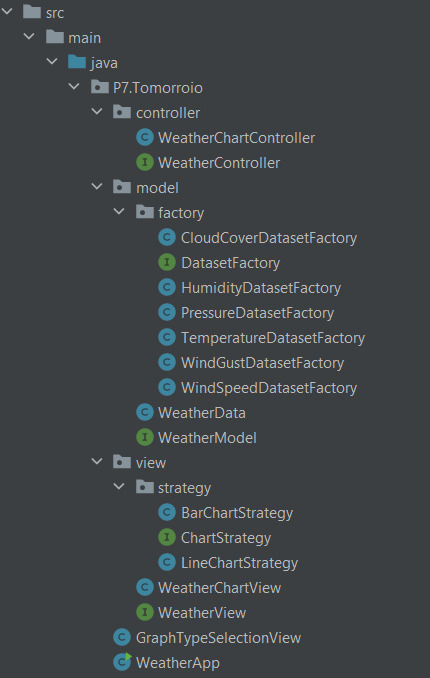
\includegraphics[width=0.8\textwidth]{images/image6.png}
  \caption{Estructura del directorio del proyecto.}
  \label{fig:estructura-proyecto}
\end{figure}

\section{Estructura del Código}
\subsection{Clase WeatherApp}
Clase principal que contiene el método main. Crea una instancia de WeatherChartController y muestra la vista.

\subsection{Clase WeatherView}
Interfaz que define el contrato para las vistas de la aplicación. Proporciona métodos para mostrar la vista y actualizar los gráficos con nuevos conjuntos de datos.

\subsubsection{Clase WeatherChartView}
Implementa la interfaz WeatherView. Crea y muestra una ventana que contiene un gráfico. Proporciona métodos para actualizar el gráfico con nuevos conjuntos de datos.

\subsection{Clase GraphTypeSelectionView}
Crea y muestra una ventana que permite al usuario seleccionar el tipo de gráfico y la ciudad. Proporciona métodos para obtener la ciudad y el tipo de gráfico seleccionados por el usuario.

\subsection{Clase ChartStrategy}
La interfaz `ChartStrategy` define el contrato para las estrategias de gráficos. A través de esta interfaz, especificamos los métodos necesarios que las estrategias concretas deben implementar para la creación de gráficos.

\subsubsection{Clase LineChartStrategy}
La clase `LineChartStrategy` implementa la interfaz `ChartStrategy`. Es una estrategia abstracta que proporciona métodos específicos para crear un gráfico de líneas utilizando JFreeChart.

\subsubsection{Clase BarChartStrategy}
La clase `BarChartStrategy` es una implementación concreta de `ChartStrategy` especializada en la creación de gráficos de barras. Hereda de `LineChartStrategy` y proporciona la implementación específica para crear gráficos de barras utilizando JFreeChart.

\subsection{Clase WeatherData}
La clase `WeatherData` implementa la interfaz `Subject` y representa un sujeto concreto en el patrón de diseño Observador. Proporciona métodos para registrar, eliminar y notificar observadores. También proporciona métodos para establecer y obtener los datos meteorológicos actuales.

\subsection{Clase DatasetFactory}
La interfaz `DatasetFactory` define el contrato para las factorías de conjuntos de datos. A través de esta interfaz, especificamos los métodos necesarios que las factorías concretas deben implementar para la creación de conjuntos de datos.

\subsubsection{Clase TemperatureDatasetFactory}
La clase `TemperatureDatasetFactory` es una implementación concreta de `DatasetFactory` especializada en la creación de conjuntos de datos para la temperatura.Proporciona la implementación específica para este tipo de dato meteorológico.

\subsubsection{Clase HumedityDatasetFactory}
La clase `HumedityDatasetFactory` implementa `DatasetFactory` y se especializa en la creación de conjuntos de datos para la humedad.  Proporciona la implementación necesaria para este tipo de dato meteorológico.

\subsubsection{Clase WindSpeedDatasetFactory}
La clase `WindSpeedDatasetFactory` es una implementación concreta de `DatasetFactory` especializada en la creación de conjuntos de datos para la velocidad del viento.Proporciona la implementación específica para este tipo de dato meteorológico.

\subsubsection{Clase PressureDatasetFactory}
La clase `PressureDatasetFactory` implementa `DatasetFactory` y se especializa en la creación de conjuntos de datos para la presión atmosférica. Proporciona la implementación necesaria para este tipo de dato meteorológico.

\subsubsection{Clase WindGustDatasetFactory}
La clase `WindGustDatasetFactory` es una implementación concreta de `DatasetFactory` especializada en la creación de conjuntos de datos para la ráfaga de viento.Proporciona la implementación específica para este tipo de dato meteorológico.

\subsubsection{Clase CloudCoverDatasetFactory}
La clase `CloudCoverDatasetFactory` implementa `DatasetFactory` y se especializa en la creación de conjuntos de datos para la cobertura de nubes. Proporciona la implementación necesaria para este tipo de dato meteorológico.


Estas clases concretas de factorías implementan métodos específicos para la creación de conjuntos de datos relacionados con sus respectivos tipos de datos meteorológicos. Al emplear el patrón Abstract Factory, logramos una estructura modular que facilita la extensión del sistema al agregar nuevos tipos de datos meteorológicos en el futuro.

\subsection{Clase WeatherChartController}
La clase `WeatherChartController` es el controlador principal de la aplicación. Implementa la interfaz `Observer` y proporciona métodos para actualizar la vista con nuevos conjuntos de datos. También proporciona métodos para obtener datos meteorológicos actualizados de `WeatherData` y crear conjuntos de datos utilizando `DatasetFactory`.

\subsection{WeatherController}
La interfaz `WeatherController` define el contrato para los controladores de la aplicación. A través de esta interfaz, especificamos los métodos necesarios que los controladores concretos deben implementar para la gestión de la aplicación.

\section{Patrones}
En esta práctica usamos varios patrones que hemos visto a lo largo de la asignatura, como puede ser el patrón estrategia, el abstract factory y el modelo de vista controlador que iremos señalando en el siguiente apartado:

\subsection{Patrón Estrategia}
El patrón de diseño Estrategia se ha utilizado para implementar diferentes tipos de gráficos. Como se puede observar en la figura \ref{fig:image2}, la clase WeatherChartView utiliza una estrategia para crear un gráfico de líneas o de barras. Esto permite que la aplicación sea flexible y extensible, ya que podemos agregar nuevos tipos de gráficos en el futuro sin modificar el código existente.

\begin{figure}[H]
  \centering
  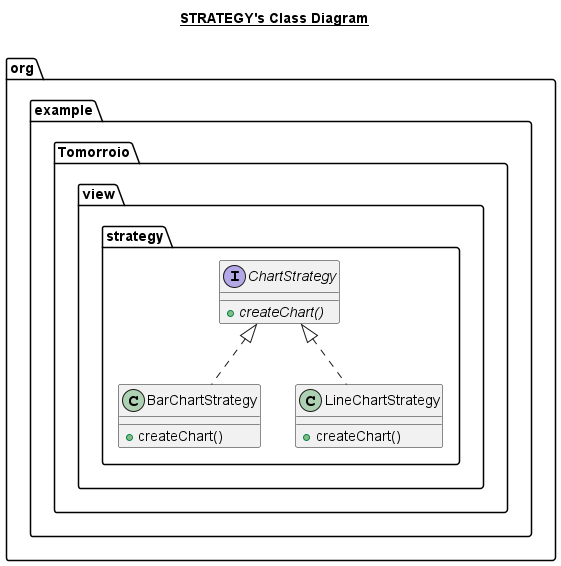
\includegraphics[width=0.8\textwidth]{images/image2.png}
  \label{fig:image2}
\end{figure}

\subsection{Patrón Abstract Factory}
El patrón de diseño Abstract Factory se ha utilizado como se puede observar en la figura \ref{fig:image7} para crear de forma dinámica los diferentes tipos de datos de forma ordenada y flexible.

\begin{figure}[H]
  \centering
  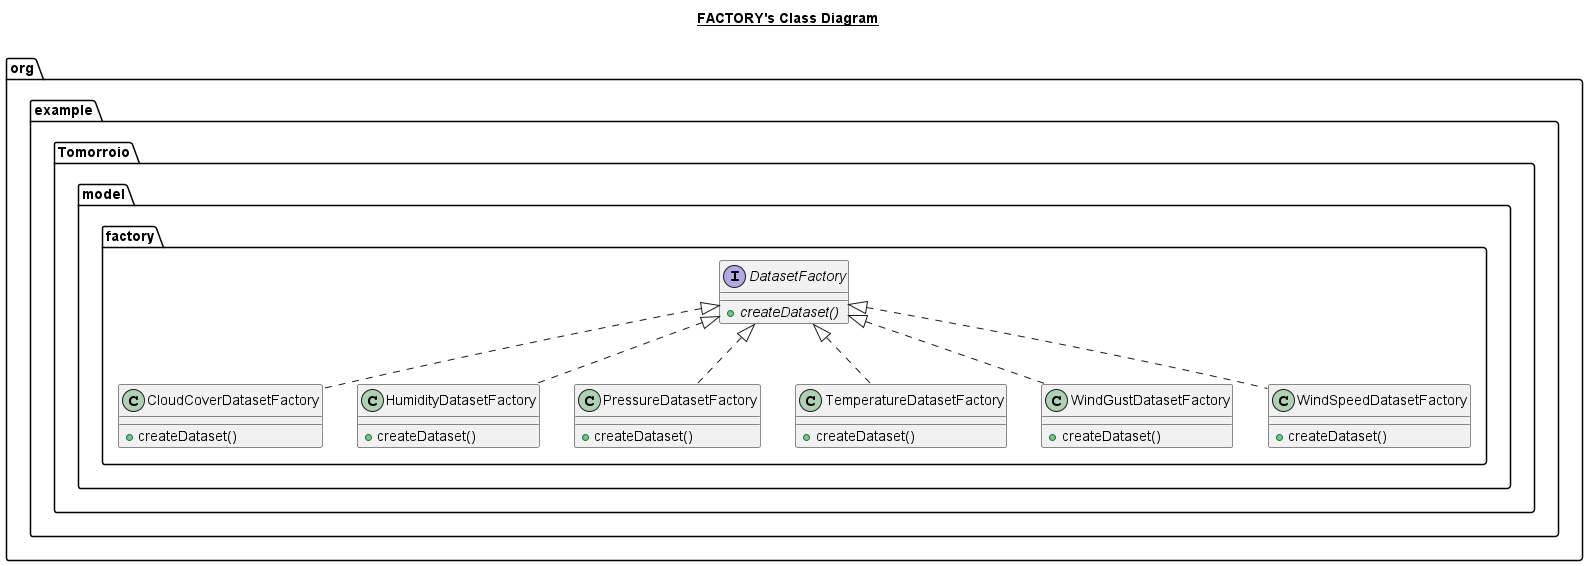
\includegraphics[width=1.1\textwidth]{images/image7.png}
  \label{fig:image7}
\end{figure}

\subsection{Patrón Modelo Vista Controlador}
El patrón de diseño Modelo Vista Controlador se ha utilizado para separar la lógica de la aplicación de la interfaz gráfica. Como se puede observar en la figura \ref{fig:image3}, la clase WeatherChartController actúa como el controlador principal de la aplicación. Implementa la interfaz WeatherController y proporciona métodos para actualizar la vista con nuevos conjuntos de datos.

\begin{figure}[H]
  \centering
  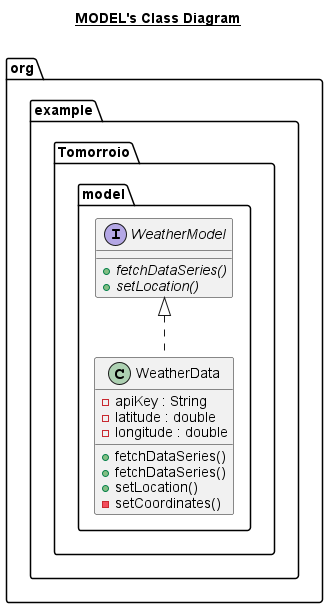
\includegraphics[width=0.5\textwidth]{images/image11.png}
  \caption {Implementación Modelo}
  \label{fig:image11}
\end{figure}

\begin{figure}[H]
  \centering
  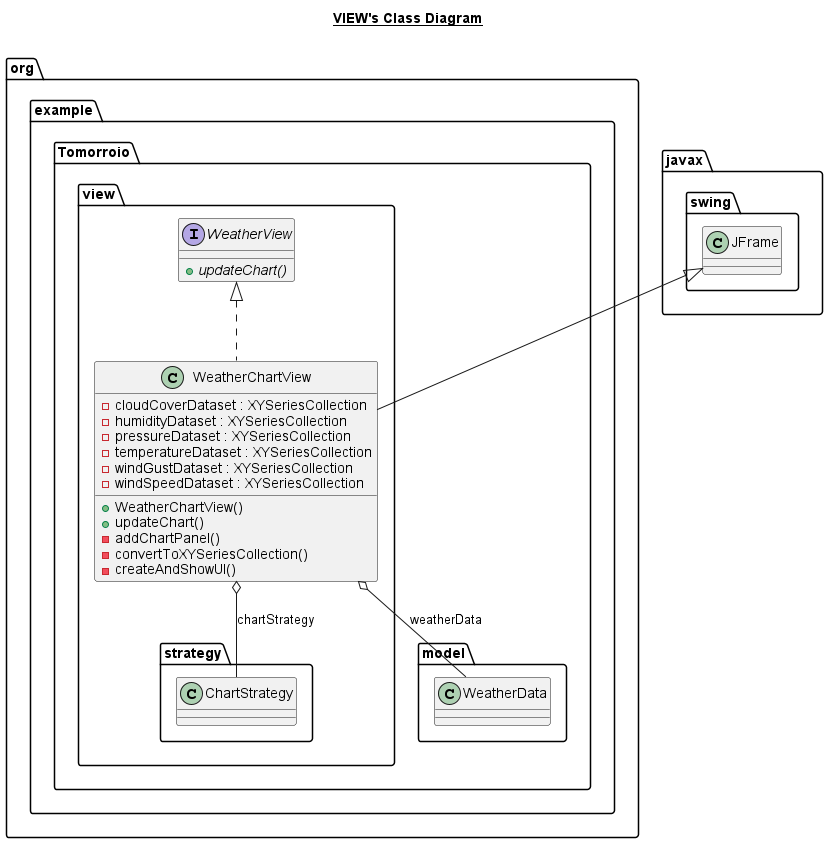
\includegraphics[width=0.6\textwidth]{images/image12.png}
  \caption {Implementación Vista}
  \label{fig:image12}
\end{figure}

\begin{figure}[H]
  \centering
  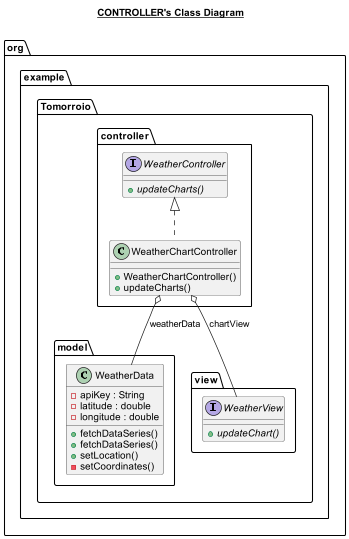
\includegraphics[width=0.5\textwidth]{images/image3.png}
  \caption {Implementación Controlador}
  \label{fig:image3}
\end{figure}

\section{Pasos del Flujo del Programa}
El programa sigue estos pasos:

\begin{enumerate}
  \item El usuario selecciona una ciudad y un tipo de gráfico.
  \item El controlador principal crea una instancia de la vista y la muestra.
  \item La vista crea una instancia de la estrategia de gráfico seleccionada por el usuario.
  \item La vista crea una instancia de la factoría de conjuntos de datos correspondiente al tipo de gráfico seleccionado por el usuario.
  \item La vista crea un gráfico utilizando la estrategia y el conjunto de datos.
  \item El controlador principal crea una instancia de WeatherData.
  \item WeatherData obtiene datos meteorológicos de la API de Tomorrow.io.
  \item El controlador principal recibe los datos meteorológicos actualizados y crea un conjunto de datos utilizando la factoría de conjuntos de datos.
  \item El controlador principal actualiza la vista con el nuevo conjunto de datos.
  \item El usuario puede seleccionar una nueva ciudad y un nuevo tipo de gráfico.
\end{enumerate}

\section{Interfaz Gráfica para el Usuario}
La interfaz gráfica para el usuario se muestra en las figuras \ref{fig:seleccion_ciudad}, \ref{fig:seleccion_ciudad2}, \ref{fig:seleccion_ciudad3} y \ref{fig:seleccion_ciudad4}.

\begin{figure}[H]
    \centering
    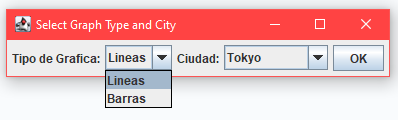
\includegraphics[width=0.5\textwidth]{images/image5.png}
    \caption{Interfaz gráfica para el usuario.}
    \label{fig:seleccion_ciudad}
\end{figure}

\begin{figure}[H]
    \centering
    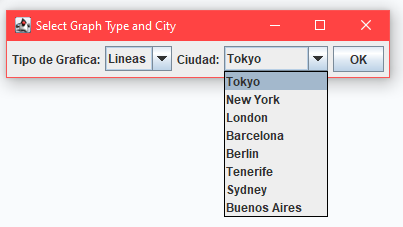
\includegraphics[width=0.7\textwidth]{images/image9.png}
    \caption{ Interfaz gráfica para el usuario.}
    \label{fig:seleccion_ciudad2}
\end{figure}

\begin{figure}[H]
  \centering
  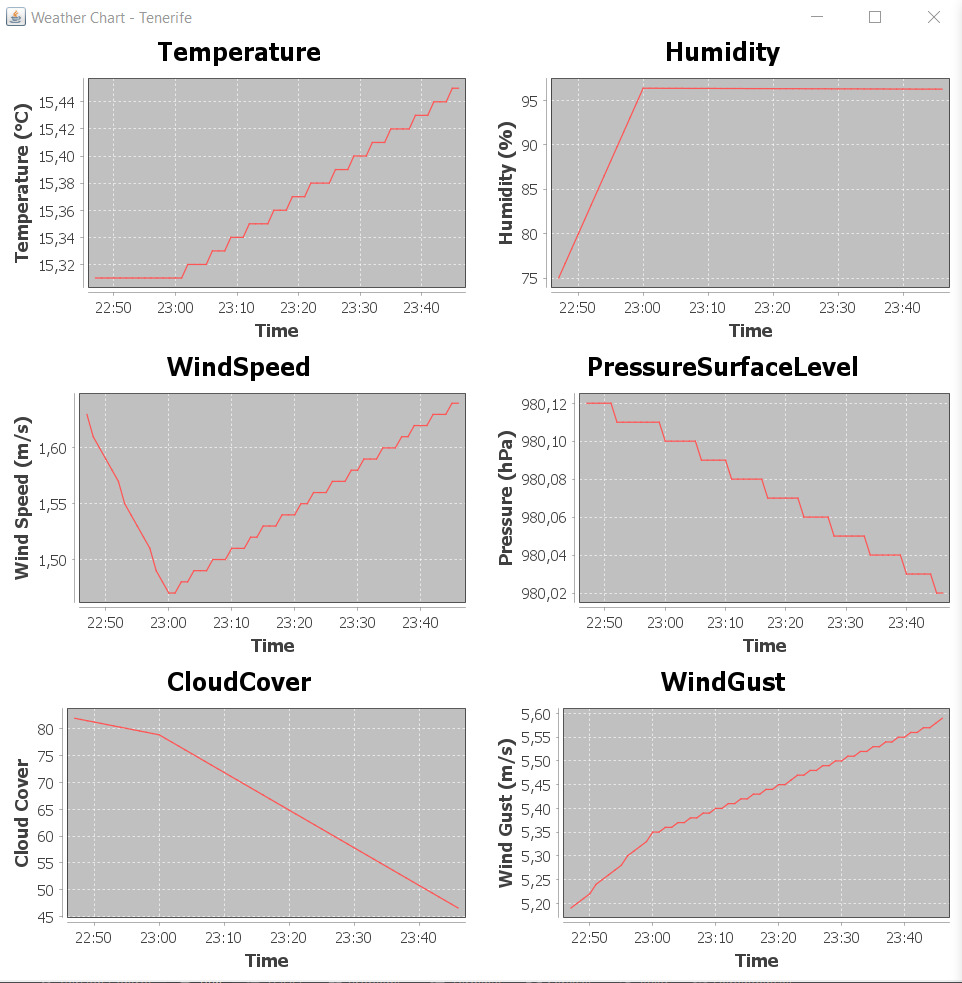
\includegraphics[width=0.7\textwidth]{images/image4.png}
  \caption{Interfaz gráfica para el usuario.}
  \label{fig:seleccion_ciudad3}
\end{figure}

\begin{figure}[H]
  \centering
  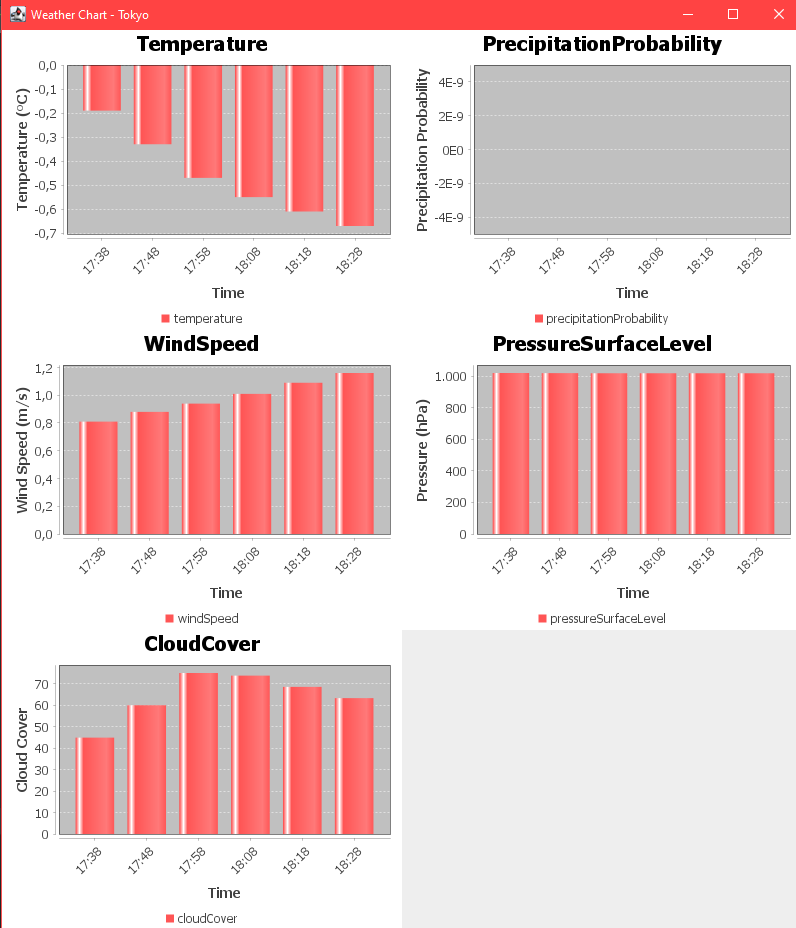
\includegraphics[width=0.7\textwidth]{images/image10.png}
  \caption{Interfaz gráfica para el usuario.}
  \label{fig:seleccion_ciudad4}
\end{figure}

\newpage 

\section{Diagrama UML}
El diagrama UML del proyecto se muestra en la Figura \ref{fig:uml}.


\begin{figure}[H]
    \centering
    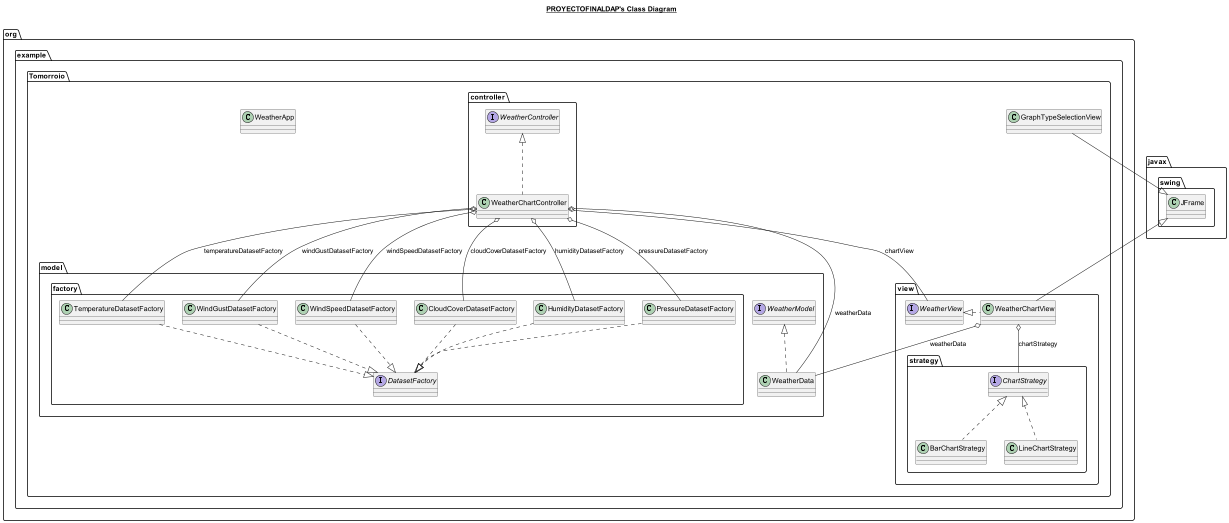
\includegraphics[width=1.0\textwidth]{images/image0.png}
    \caption{Diagrama UML del proyecto.}
    \label{fig:uml}
\end{figure}

\section{Errores y Desafíos Encontrados}
Durante el desarrollo del proyecto, nos enfrentamos a varios desafíos que nos permitieron mejorar nuestras habilidades de resolución de problemas y fortalecer la calidad general del sistema.

\subsection{Conexión con la API de Tomorrow.io}
Uno de los desafíos iniciales fue establecer una conexión efectiva con la API de Tomorrow.io para obtener datos meteorológicos en tiempo real. En algunos casos, experimentamos problemas de tiempo de espera y errores de conexión. Para superar esto, implementamos un manejo robusto de errores y optimizamos nuestras solicitudes para mejorar la eficiencia.

\subsection{Sincronización de Datos en Tiempo Real}
La sincronización de datos en tiempo real para proporcionar actualizaciones constantes en la interfaz gráfica fue un desafío importante. Implementamos un mecanismo de actualización basado en eventos para garantizar que los gráficos reflejaran con precisión los datos meteorológicos más recientes. Esto implicó coordinar eficientemente la obtención de datos, su procesamiento y la actualización de la interfaz de usuario.

\subsection{Manejo de Excepciones}
En el proceso de desarrollo, identificamos la necesidad de un manejo exhaustivo de excepciones para garantizar la estabilidad y la usabilidad de la aplicación. Implementamos una estrategia sólida de manejo de excepciones para notificar al usuario sobre posibles problemas y evitar fallos inesperados.

Estos desafíos contribuyeron significativamente a nuestro aprendizaje y resiliencia durante el desarrollo del proyecto. La capacidad para superar estos obstáculos mejoró nuestras habilidades de resolución de problemas y fortaleció la calidad general del sistema.

\section{Estimación de Plazo}
\begin{table}[H]
  \centering
  \caption{Estimación de Plazo}
  \begin{tabular}{|c|c|c|}
    \hline
    \textbf{Tarea} & \textbf{Tiempo Estimado} & \textbf{Tiempo Real} \\
    \hline
    Elegir propuesta & 30 minutos & 15 minutos \\
    Implementar JFreeChart & 3 hora & 5 hora y media \\
    Obtener datos historial & 30 minutos & 50 minutos \\
    Implementar patrones & 1 hora & 2 horas \\
    Implementar interfaces & 2 horas & 2 horas y media \\
    Pruebas y depuración & 2 horas & 3 horas \\
    Documentación & 1 hora & 1 hora y media \\
    Implementación Github & 1 hora y media & 1 hora y media \\
    \hline
  \end{tabular}
  \label{Estimación de Plazo}
\end{table}

\section{Conclusiones}
En conclusión, el uso de patrones de diseño ha simplificado el diseño y la implementación de la aplicación. Ha proporcionado una estructura modular y extensible, facilitando la incorporación de nuevas funcionalidades en algún futuro. Además de utilizar diferentes herramientas, como el JFreeChart, para realizar un proyecto bastante práctico y elaborado.

\section{Bibliografía}
\begin{thebibliography}{99}
    \bibitem Tomorrow.io API: \url{https://www.tomorrow.io/}
    \bibitem JFreeChart: \url{https://www.jfree.org/jfreechart/}
    \bibitem JFreeChart Developer Guide: \url{https://www.jfree.org/jfreechart/api/javadoc/org/jfree/chart/JFreeChart.html}
    \bibitem JFreeChart Tutorial: \url{https://www.tutorialspoint.com/jfreechart/index.htm}
    \bibitem JFreeChart Tutorial: \url{https://www.tutorialspoint.com/jfreechart/jfreechart_quick_guide.htm}
    \bibitem JFreeChart Tutorial: \url{https://www.tutorialspoint.com/jfreechart/jfreechart_overview.htm}
    \bibitem JFreeChart Tutorial: \url{https://www.tutorialspoint.com/jfreechart/jfreechart_xy_chart.htm}
    \bibitem JFreeChart Tutorial: \url{https://www.tutorialspoint.com/jfreechart/jfreechart_bar_chart.htm}
    \bibitem JFreeChart Tutorial: \url{https://www.tutorialspoint.com/jfreechart/jfreechart_line_chart.htm}
    \bibitem JFreeChart Tutorial: \url{https://www.tutorialspoint.com/jfreechart/jfreechart_pie_chart.htm}
    \bibitem WeatherStack API: \url{https://weatherstack.com/}
    \bibitem atrones de diseño: \url{https://www.tutorialspoint.com/design_pattern/index.htm}
    \bibitem Patrones de diseño: \url{https://www.geeksforgeeks.org/software-design-patterns/}
    \bibitem Patrones de diseño: \url{https://www.journaldev.com/1827/java-design-patterns-example-tutorial}
    \bibitem Patrones de diseño: \url{https://www.javatpoint.com/design-patterns-in-java}
\end{thebibliography}

\end{document}